\subsection{Présentation}

Ce projet de TER prolonge un travail déjà entamé l'année dernière par deux étudiants de Polytech, consistant à enregistrer en vidéo l'écriture d'un calligraphe, pour pouvoir reconstruire un modèle en 3D du mouvement de la plume. Une structure en bois supporte deux caméras, que l'on peut bouger le long de rails puis fixer à l'aide de vis (Figure \ref{cameras}). Le calligraphe écrit sous cette structure et la feuille est éclairée par des spots lumineux. Il faut alors associer l'image des deux caméras, ce qui n'est pas possible nativement avec le logiciel fourni par le fabricant (FlyCapture de PointGrey) pour faire de l'acquisition vidéo en stéréo, puis reconstituer via OpenGL les mouvements de la plume. Ces mouvements ont été sauvegardés grâce à des algorithmes de tracking, travaillant sur les vidéos enregistrées auparavant.

\begin{figure}[!h]
\centering
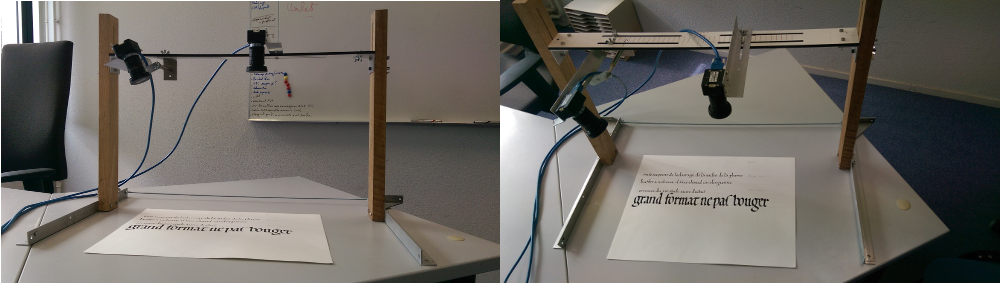
\includegraphics[width=\textwidth, height=4cm]{Modules/Picture/camerasPic.png}
\caption{Dispositif de capture stéréo}
\label{cameras}
\end{figure}


\subsection{But du projet}

Ce projet permettra à terme de réaliser une reconstitution 3D des mouvements du calligraphe. On pourra alors lui faire recopier plusieurs textes, provenant de différents lieux et différentes époques, afin de pouvoir comparer les styles d'écriture, définir s'il existait différentes écoles d'écriture, différents styles, etc. De manière plus générale, le projet pourra servir pour beaucoup d'applications par la suite, car le code final se voudra le plus généraliste possible.